% ============================================================================
% Accessibility
% ============================================================================
\DocumentMetadata{
  lang = en-US, 
  pdfstandard = ua-2, 
  tagging = on, 
  tagging-setup = {math/setup=mathml-SE}
}

% ============================================================================
% Document Properties - used on title slide and PDF metadata fields
% ============================================================================
\def\PresTitle{Surface Roughness}  % Required - top line of title slide
\def\PresSubtitle{Gauges and Measurement}         % Optional - second line
\def\PresAuthor{Brad Peirson}               % Required - below dividing line
\def\PresInstitute{College of Information Technology and Engineering}       % Optional
\def\PresDate{}                             % Optional
\def\PresKeywords{}                         % Optional - used for hyperref

% Presentation Formatting
% ============================================================================
% ============================================================================
% Class Declaration
% ============================================================================
\documentclass[
        mode = handout,     % Projector = one bullet at a time, Handout = all
        font-size=14pt,     % Only accepts 9, 10, 12, 14, 17, 20
        pdfusetitle         % Pulls \title property from document
    ]
    {ltx-talk}              % ltx-talk class

% ============================================================================
% Custom Colors
% ============================================================================
\usepackage[table]{xcolor}
% Colors from the Baker College Style Guide
%\definecolor{BakerADARed}{RGB}{231, 0, 46}   % #e7002e Official ADA red-doesn't pass WCAG AAA for small text
\definecolor{BakerADARed}{RGB}{181, 0, 36}    % #b50024 Adjusted ADA red-passes WCAG AAA for small text
\definecolor{HoneyYellow}{RGB}{255, 196, 0}   % #ffc400
\definecolor{UpNorthGreen}{RGB}{114, 191, 68} % #72bf44
\definecolor{LakeBlue}{RGB}{134, 183, 227}    % #86b7e3
\definecolor{BakerADI}{RGB}{58, 98, 170}
\definecolor{BakerCIM}{RGB}{217, 35, 47}
\definecolor{BakerBlack}{RGB}{31, 34, 40}     % #1f2228
\definecolor{BakerWhite}{RGB}{255, 255, 255}
\definecolor{BakerRed}{RGB}{239, 0, 48}
\definecolor{Abbey}{RGB}{80, 82, 88}
\definecolor{RollingStone}{RGB}{121, 124, 126}
\definecolor{HitGray}{RGB}{165, 169, 172}
\definecolor{Iron1}{RGB}{201, 206, 209}
\definecolor{Iron}{RGB}{222, 225, 226}
\definecolor{BlackHaze1}{RGB}{237, 240, 240}
\definecolor{BlackHaze}{RGB}{245, 247, 247}

% ============================================================================
% Document Data
% ============================================================================
\title{\PresTitle}
\author{\PresAuthor}
\institute{\PresInstitute}
\date{\PresDate}

%Set up the hyperlink colors
\hypersetup{colorlinks,
    linkcolor=BakerBlack,
    urlcolor=BakerADARed,
    pdfauthor = {\PresAuthor},
    %pdftitle = {\PresentationTopic},   % Title is pulled directly
    pdfsubject = {\PresSubtitle},
    pdfkeywords = {\Keywords},
    pdfcreator = {LaTeX with hyperref package},
    pdfproducer = {LuaLaTeX}
    }

% Map your custom style guide colors to the progress bar aliases
\colorlet{pbcomplete}{BakerADARed}
\colorlet{pbincomplete}{Iron}

\usepackage[most]{tcolorbox}

% ============================================================================
% Footer Format
% ============================================================================
\EditInstance{footer}{std}{
  color         = Abbey,
  separator     = \hfill,
  element-order = {title, institute, framenumber},
  right-hspace  = 3mm,
  left-hspace   = 3mm,
}

% \DeclareInstance{footer}{empty}{
%   element-order = {}
% }

% ============================================================================
% Progress Bar Toggles & Helper Macros
% ============================================================================
\usepackage{xfp}        % Needed for floating point math
\newif\ifprogressbar    % Used to determine whether or not to show the bar
\progressbartrue        % Set the bar to true at the start

% Helper macro to automatically turn off the progress bar inside title/section frames
\newcommand{\makeblindframe}[1]{%
  \progressbarfalse
  #1%
  \progressbartrue
}

% ============================================================================
% Custom Page Formats
% ============================================================================
\let\oldmaketitle\maketitle         % Backup the original maketitle command
\let\oldsection\section             % Backup the original section command
\let\oldsubsection\subsection       % Backup the original subsection command

\makeatletter
\renewcommand{\maketitle}{%
\makeblindframe{%
  \disableglobalbackground
  \slidebackground{PresentationTitleGraphic_2048x1151}%
  \color{white}%
  %\UseInstance{footer}{wallpaper}
  \begin{frame}
    \vspace*{1in}%
      \begin{tcolorbox}[
          enhanced,
          colback=black,       
          colframe=black,      
          opacityfill=0.25,       
          arc=6pt,                
          boxrule=0pt,            
          left=20pt, right=20pt,  
          top=20pt, bottom=20pt,
          width=0.80\textwidth,   
          halign=left             
      ]
          \color{white}%
          % Title (Always visible)
          {\large\bfseries\sffamily \@title}\\[0.5em]%
          
          % Conditional Subtitle
          \ifx\PresSubtitle\empty
          \else
            {\normalsize\sffamily \PresSubtitle}\\[0.5em]%
          \fi
          
          % High-contrast divider line
          {\color{white!80}\rule{0.3\textwidth}{0.8pt}}\\[0.5em]%
          
          % Author (Always visible)
          {\small\sffamily \@author}\\%
          
          % Conditional Institute
          \ifx\PresInstitute\empty
          \else
            {\small\sffamily \PresInstitute}\\%
          \fi
          
          % Conditional Date
          \ifx\PresDate\empty
          \else
            {\small\sffamily \@date}\\%
          \fi
      \end{tcolorbox}%
      \vfill     
  \end{frame}%
  \enableglobalbackground{BG}%
  \color{black}%
  %\UseInstance{footer}{std}
}%
}
\makeatother

% Create a variable container to hold the current section title
\newcommand{\currentsectiontitle}{}

% Redefine \section to take 1 argument (the title)
\renewcommand{\section}[1]{%
\makeblindframe{%
  \renewcommand{\currentsectiontitle}{#1}%
  \disableglobalbackground
  \slidebackground{PresentationSectionBackground_2048x1151}%
  \begin{frame}
    \vfill
    %\vspace*{0.625in}%
    \begin{tcolorbox}[
        enhanced,
        colback=black,       
        colframe=black,      
        opacityfill=0.25,       
        arc=6pt,                
        boxrule=0pt,            
        left=20pt, right=20pt,  
        top=20pt, bottom=20pt,
        width=0.80\textwidth,   
        halign=left             
    ]
        \color{white}%
        {\large\bfseries\sffamily #1}\\[0.5em]%   
    \end{tcolorbox}%
    \vfill 
  \end{frame}%
  \oldsection{#1}%
  \enableglobalbackground{BG}%

  % This will be used for an auto TOC at every section
  % Right now ltx-talk TOC is still in development
  % Once it comes a little further along this can be used
  % \begin{frame}
  %       \frametitle{Section Overview}
  %       \tableofcontents[sections=\thesection]
  %   \end{frame}%
}%
}

% Redefine \subsection to take 1 argument
\renewcommand{\subsection}[1]{%
\makeblindframe{%
  \disableglobalbackground
  \slidebackground{PresentationSectionBackground_2048x1151}%
  \begin{frame}
    \vfill
    %\vspace*{0.25in}% 
    \begin{tcolorbox}[
        enhanced,
        colback=black,       
        colframe=black,      
        opacityfill=0.25,       
        arc=6pt,                
        boxrule=0pt,            
        left=20pt, right=20pt,  
        top=20pt, bottom=20pt,
        width=0.80\textwidth,   
        halign=left             
    ]
        \color{white}%
        {\large\bfseries\sffamily\currentsectiontitle}\\[0.5em]%
        {\normalsize\sffamily #1}%
    \end{tcolorbox}%
    \vfill 
  \end{frame}%
  \oldsubsection{#1}%
  \enableglobalbackground{BG}%
}%
}

%Set the fonts to use NeueHaas Grotesk
\setsansfont{NHAASGROTESKTXPRO-}[
    Path=../NeueHaasGroteskFiles/,
    Scale=1.0,
    Extension = .ttf,
    UprightFont=*55Rg,
    BoldFont=*75Bd,
    ItalicFont=*56It,
    BoldItalicFont=*76BdIt
    ]

% Force the document default family to Sans-Serif
\renewcommand{\familydefault}{\sfdefault}

\usepackage{mathtools} % Load BEFORE unicode math settings
\setmathfont{Fira Math}[Scale=MatchLowercase] 

% 1. Turn global background ON
\newcommand{\enableglobalbackground}[1]{%
  \AddToHook{shipout/background}[mybg]{%
    \put(0, -\paperheight){%
      \includegraphics[width=\paperwidth, height=\paperheight, artifact]{#1}%
    }%
  }%
}

% 2. Turn global background OFF
\newcommand{\disableglobalbackground}{%
  \RemoveFromHook{shipout/background}[mybg]%
}

\newcommand{\slidebackground}[1]{%
  \AddToHookNext{shipout/background}{%
    \put(0, -\paperheight){%
      \includegraphics[width=\paperwidth, height=\paperheight, artifact]{#1}%
    }%
  }%
}

% --- GLOBAL BULLET OVERRIDES ---
\renewcommand{\labelitemi}{\color{BakerBlack}\Large\textbullet}
\renewcommand{\labelitemii}{\color{BakerBlack}\large\textbullet}
\renewcommand{\labelenumi}{\color{BakerBlack}\bfseries\arabic{enumi}.}
\renewcommand{\labelenumii}{\color{BakerBlack}\bfseries\alph{enumii})}

\AddToHook{begindocument/before}{%
  \EditInstance{item}{description}{
    label-format = \normalfont\bfseries\color{BakerADARed}#1
  }%
}

\AddToHook{begindocument/before}{%
  \EditInstance{item}{basic}{
    label-format = \color{BakerADARed}#1
  }%
}

% Global override for ltx-talk slide titles
\EditInstance{frametitle}{header}{
    font = \rule{0pt}{1.5cm}\bfseries\Large,
}

\EditInstance{header}{std}{
    font = \bfseries\huge,
    color = BakerBlack,
}

\AddToHook{env/block/begin}{%
  \colorlet{structure}{BakerADARed}%
}

\pretocmd{\tableofcontents}{\begin{minipage}{\textwidth} \linespread{1.4}}{}{}
\apptocmd{\tableofcontents}{\end{minipage}}{}{}

%Biber not functional in ltx-talk as of 2026-05-29
%Package that allows the creation of bibliographies
\usepackage[
    backend=biber,
    style=authoryear,
    sorting=none,
    %entryhead=false
    ]{biblatex}

%Load the bibliography file
\addbibresource{../../reference.bib}

\defbibheading{bibslide}{References}

\newcolumntype{L}[1]{>{\raggedright\let\newline\\\arraybackslash\hspace{0pt}}m{#1}}
\newcolumntype{C}[1]{>{\centering\let\newline\\\arraybackslash\hspace{0pt}}m{#1}}
\newcolumntype{R}[1]{>{\raggedleft\let\newline\\\arraybackslash\hspace{0pt}}m{#1}}

%All of the graphics are in a seperate folder, this makes it so the folder doesn't have to be repeated every time
\graphicspath{
  {../assets/images}
  {../assets/diagrams}
  {../assets/plots}
}

\makeatletter
% New counter to hold the custom "max frames" for the progress bar
\newcommand{\pb@maxtotal}{1}

% Read the custom total from the .aux file if it exists
\AtBeginDocument{%
  \ifdefined\pb@storedtotal
    \let\pb@maxtotal\pb@storedtotal
  \else
    % Fallback to standard total if our custom hook hasn't run yet
    \edef\pb@maxtotal{\@totalframes}%
  \fi
}

% Custom Appendix command that caps the progress bar and turns it off
\newcommand{\talkappendix}{%
  % 1. Write the CURRENT frame number to the .aux file as the progress total
  \immediate\write\@auxout{\string\gdef\string\pb@storedtotal{\@framenumber}}%
  % 2. Turn off the progress bar for all subsequent appendix slides
  \progressbarfalse
}
\makeatother

% ============================================================================
% Progress Bar Logic 
% ============================================================================
\makeatletter               
\AddToHook{shipout/background}{%
  \ifprogressbar
    % Read ltx-talk's internal frame counter safely
    \edef\currentframe{\@framenumber}%
    \edef\totalframes{\pb@maxtotal}% Use our custom max total instead
    
    % Fallback checks: If the document hasn't fully compiled yet, default to 1
    \ifx\currentframe\empty\def\currentframe{1}\fi
    \ifx\totalframes\empty\def\totalframes{1}\fi
    
    % Draw the progress bar if we have a valid total frame count
    \ifnum\totalframes>1\relax
      % Compute fraction width: (current - 1) / (total - 1)
      \edef\pbfraction{\fpeval{(\currentframe - 1) / (\totalframes - 1)}}%
      
      % Guard rails to prevent the bar from overshooting 100% on a first compile
      \ifdim\pbfraction pt>1pt\def\pbfraction{1}\fi 
      
      \edef\completewidth{\fpeval{\pbfraction * \paperwidth}}%
      \edef\incompletewidth{\fpeval{\paperwidth - \completewidth}}%
      
      % Render full-width progress bar at the top edge
      \put(0cm, -0.1cm){%
        \color{pbcomplete}\rule{\completewidth pt}{2pt}%
        \color{pbincomplete}\rule{\incompletewidth pt}{2pt}%
      }%
    \fi
  \fi
}
\makeatother

% 1. Globally shrink all caption components right as the caption engine fires
\AddToHook{cmd/@makecaption/before}{\footnotesize}

% 2. Declare and assign a blank plug to the kernel's caption label socket
\NewSocketPlug{caption/label}{nolabel}{}
\AssignSocketPlug{caption/label}{nolabel}

\usepackage{adjustbox}

\usepackage{amssymb}
\usepackage{amsmath}
\usepackage{siunitx}

\usepackage{animate}

\usepackage{calc} % Optional, but helpful for layout

\usepackage{multirow}

\usepackage{textcomp}

\usepackage{booktabs}
\usepackage{tabularx}

\usepackage[americanvoltages]{circuitikz}
\usepackage{pgfplots}
\usepackage{pgf-pie}

\usetikzlibrary{
    intersections, 
    fillbetween,
    patterns,
    decorations.pathreplacing,
    decorations.pathmorphing,
    decorations.text,
    decorations.markings,
    arrows.meta,
    arrows,
    shapes,
    shapes.geometric,
    shadows,
    calligraphy,
    backgrounds,
    intersections,
    calc,
    math,
    positioning,
    svg.path,
    shadows,
    shadows.blur,
    spy,
    }

\pgfplotsset{compat=1.18}

\pgfdeclarelayer{ft}
\pgfdeclarelayer{bg}
\pgfsetlayers{bg, main, ft}

% Usage: \hexpic[]{height}{Alt text}{Attribution}{image path}
\newcommand{\hexpic}[5][]{%
  \begin{figure}
    \centering
    \begin{tikzpicture}[
      baseline=(hex.base),      
      every shadow/.style={
        shadow opacity=70
        }
      ]
      \node (hex) [
        draw=white, 
        minimum size=#2, 
        regular polygon, 
        regular polygon sides=6, 
        rotate=90,
        blur shadow
      ] {};
      \begin{scope}
        \clip (hex.corner 1) -- (hex.corner 2) -- (hex.corner 3) -- 
              (hex.corner 4) -- (hex.corner 5) -- (hex.corner 6) -- cycle;
        \node at (hex.center) [#1] {
          \includegraphics[height=#2, alt={#3}]{#5}
        };
      \end{scope}
    \end{tikzpicture}

    \vspace{0.5em}
    {\tiny #4\par}
  \end{figure}  
}

% Usage: \shadowpic[]{width}{Alt text}{Attribution}{image path}
\newcommand{\shadowpic}[5][]{%
  \begin{figure}
    \centering
    \begin{tikzpicture}
      [every shadow/.style={
        shadow opacity=70
        }
      ]
      \node (image) [
        inner sep=0,
        blur shadow
      ] {\includegraphics[width=#2, alt={#3}]{#5}};
    \end{tikzpicture}

    \vspace{0.5em}
    {\tiny #4\par}
  \end{figure}
}

\tikzset{middlearrow/.style={
        decoration={markings, 
        mark= at position 0.5 with {\arrow{#1}},
        },
        postaction={decorate}
    }
}

% Usage: \tikztodo[width]{height}{description/notes}
\newcommand{\tikztodo}[3][0.8\textwidth]{%
  \begin{center}
    \fbox{%
      \parbox[c][#2][c]{#1}{%
        \centering
        \textbf{\textcolor{red}{TODO: TikZ Diagram}}\\[0.5em]
        \small #3%
      }%
    }%
  \end{center}%
}

% Macro: \drawrails{<number_of_1cm_segments>}
\newcommand{\drawrails}[1]{
  % Calculate total depth: 1 cm per segment
  \pgfmathsetmacro{\railheight}{-1 * #1}
  
  % L1 Rail (x = 0)
  \draw[thick] (0, 0) -- (0, \railheight cm);
    
  % L2 Rail (x = 15)
  \draw[thick] (15, 0) -- (15, \railheight cm);
}

\newcommand{\ccwplus}{%
  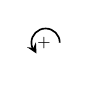
\begin{tikzpicture}[baseline=(char.base)]
    \node(char) at (0,0) {\(\scriptscriptstyle +\)};
    \draw[->, >=stealth, semithick] (0.2,0) arc (0:230:0.18cm);
  \end{tikzpicture}%
}

%====================================================================================
% Timer Ladder Symbol - Could be used for TON, TOF, RTO....
%====================================================================================
\tikzset{
    TON/.pic={

        \draw[
          BakerBlack
        ]
        (0,0)
        -- ++(0,0.375)
        -- ++(3.5,0)
        coordinate[pos=0.5](-TOP)
        -- ++(0,-1.75)
        coordinate[pos=3/14](-OUT)
        coordinate[pos=0.5](-EN1)
        coordinate[pos=0.875](-DN1)
        -- ++(-3.5,0)        
        -- (0,0)
        coordinate(-IN);

        \node[
          text=BakerBlack,
          font=\bfseries,
          anchor=east
        ](pre)
        at ($(-TOP)-(0,1.75em)$)
        {{\small PRE:}};

        \node[
          text=BakerBlack,
          font=\bfseries,
          anchor=east
        ](acc)
        at ($(pre.east)-(0,1em)$)
        {{\small ACC:}};

        \coordinate (-PRE) at (pre.east); % For the preset value
        \coordinate (-ACC) at (acc.east);

        \draw[
            BakerBlack
        ]
        (-EN1)
        -- ++(0.5,0)
        coordinate(-EN2)
        node[
            text=BakerBlack,
            anchor=west
        ]
        {{\small EN}};

        \draw[
            BakerBlack
        ]
        (-DN1)
        -- ++(0.5,0)
        coordinate(-DN2)
        node[
            text=BakerBlack,
            anchor=west
        ]
        {{\small DN}};

    }
}

%====================================================================================
% Oval ladder symbol, good for ONS, RES, etc.
%====================================================================================
\tikzset{
    ONS/.pic={

        \draw[
          BakerBlack
        ]
        (0,0)
        coordinate(-IN)
        -- ++(0.75,0)
        node[
          draw=BakerBlack, 
          text=BakerBlack, 
          font=\small, 
          minimum width=1.5cm, 
          minimum height=0.75cm, 
          anchor=west, 
          rounded corners=0.25cm
          ](ons){};
        
        \draw[BakerBlack] (ons.east) -- ++(0.75,0) coordinate(-OUT);

        \coordinate(-INS) at (ons.center);
        \coordinate(-VAR) at (ons.north); 
    }
}

%====================================================================================
% Source A, Source B, Dest box
%====================================================================================
\tikzset{
    SrcDest/.pic={
      
        \draw[
          BakerBlack
        ]
        (0,0)
        coordinate(-IN)
        -- ++(0,0.375)
        -- ++(5,0)
        coordinate[pos=0.5](-TOP)
        -- ++(0,-3.25)
        coordinate[pos=3/26](-OUT)
        -- ++(-5,0)
        -- (0,0)
        coordinate(l1);

        \node[
          text=BakerBlack,
          font=\bfseries,
          anchor=west
        ](srcA)
        at (l1)
        {{\small Src A:}};

        \node[
          text=BakerBlack,
          font=\bfseries,
          anchor=west
        ](srcB)
        at ($(l1)-(0,2em)$)
        {{\small Src B:}};

        \node[
          text=BakerBlack,
          font=\bfseries,
          anchor=west
        ](dest)
        at ($(srcB.west)-(0,2em)$)
        {{\small Dest:}};

        \coordinate(-SRCA) at (srcA.east);
        \coordinate(-AVAL) at ($(srcA.east)-(0,1em)$);
        \coordinate(-SRCB) at (srcB.east);
        \coordinate(-BVAL) at ($(srcB.east)-(0,1em)$);
        \coordinate(-DEST) at ($(-BVAL)-(0,1em)$);
        \coordinate(-DVAL) at ($(-DEST)-(0,1em)$);
    }
}

%====================================================================================
% Source A, Source B box
%====================================================================================
\tikzset{
    SrcAB/.pic={
      
        \draw[
          BakerBlack
        ]
        (0,0)
        coordinate(-IN)
        -- ++(0,0.375)
        -- ++(4,0)
        coordinate[pos=0.5](-TOP)
        -- ++(0,-2.25)
        coordinate[pos=1/6](-OUT)
        -- ++(-4,0)
        -- (0,0)
        coordinate(l1);

        \node[
          text=BakerBlack,
          font=\bfseries,
          anchor=west
        ](srcA)
        at (l1)
        {{\small Src A:}};

        \node[
          text=BakerBlack,
          font=\bfseries,
          anchor=west
        ](srcB)
        at ($(l1)-(0,2em)$)
        {{\small Src B:}};

        \coordinate(-SRCA) at (srcA.east);
        \coordinate(-AVAL) at ($(srcA.east)-(0,1em)$);
        \coordinate(-SRCB) at (srcB.east);
        \coordinate(-BVAL) at ($(srcB.east)-(0,1em)$);
    }
}

%====================================================================================
% LIMIT instruction
%====================================================================================
\tikzset{
    Limit/.pic={
      
        \draw[
          BakerBlack
        ]
        (0,0)
        coordinate(-IN)
        -- ++(0,0.375)
        -- ++(4,0)
        coordinate[pos=0.5](-TOP)
        -- ++(0,-3.25)
        coordinate[pos=3/26](-OUT)
        -- ++(-4,0)
        -- (0,0)
        coordinate(l1);

        \node[
          text=BakerBlack,
          font=\bfseries,
          anchor=west
        ](srcA)
        at (l1)
        {{\small Low:}};

        \node[
          text=BakerBlack,
          font=\bfseries,
          anchor=west
        ](srcB)
        at ($(l1)-(0,2em)$)
        {{\small Test:}};

        \node[
          text=BakerBlack,
          font=\bfseries,
          anchor=west
        ](dest)
        at ($(srcB.west)-(0,2em)$)
        {{\small High:}};

        \coordinate(-LO) at (srcA.east);
        \coordinate(-LOV) at ($(srcA.east)-(0,1em)$);
        \coordinate(-TEST) at (srcB.east);
        \coordinate(-TESTV) at ($(srcB.east)-(0,1em)$);
        \coordinate(-HI) at ($(-TESTV)-(0,1em)$);
        \coordinate(-HIV) at ($(-HI)-(0,1em)$);
    }
}

%====================================================================================
% Source Destination box
%====================================================================================
\tikzset{
    SrcSingle/.pic={
      
        \draw[
          BakerBlack
        ]
        (0,0)
        coordinate(-IN)
        -- ++(0,0.375)
        -- ++(6,0)
        coordinate[pos=0.5](-TOP)
        -- ++(0,-2.25)
        coordinate[pos=1/6](-OUT)
        -- ++(-6,0)
        -- (0,0)
        coordinate(l1);

        \node[
          text=BakerBlack,
          font=\bfseries,
          anchor=west
        ](srcA)
        at (l1)
        {{\small Source:}};

        \node[
          text=BakerBlack,
          font=\bfseries,
          anchor=east
        ](srcB)
        at ($(srcA.east)-(0,2em)$)
        {{\small Dest:}};

        \coordinate(-SRC) at (srcA.east);
        \coordinate(-SRCV) at ($(srcA.east)-(0,1em)$);
        \coordinate(-DEST) at (srcB.east);
        \coordinate(-DESTV) at ($(srcB.east)-(0,1em)$);
    }
}

%====================================================================================
% Compute Box
%====================================================================================
\tikzset{
    CPT/.pic={
      
        \draw[
          BakerBlack
        ]
        (0,0)
        coordinate(-IN)
        -- ++(0,0.375)
        -- ++(8.5,0)
        coordinate[pos=0.5](-TOP)
        -- ++(0,-1.75)
        coordinate[pos=3/14](-OUT)
        -- ++(-8.5,0)
        -- (0,0)
        coordinate(l1);

        \node[
          text=BakerBlack,
          font=\bfseries,
          anchor=west
        ](srcA)
        at (l1)
        {{\small Source:}};

        \node[
          text=BakerBlack,
          font=\bfseries,
          anchor=east
        ](srcB)
        at ($(srcA.east)-(0,2em)$)
        {{\small Exp:}};

        \coordinate(-DEST) at (srcA.east);
        \coordinate(-DESTV) at ($(srcA.east)-(0,1em)$);
        \coordinate(-EXP) at (srcB.east);
        \coordinate(-EXPV) at ($(srcB.east)-(0,1em)$);
    }
}

% ============================================================================
% Document Content
% ============================================================================
\begin{document}

\maketitle              % Redefined in the preamble to generate a full frame

\begin{frame}
    \frametitle{Agenda}
    \begingroup
        % Tighten the spacing between paragraphs/TOC lines
        \setlength{\parskip}{0.3em} 
        
        % Optionally tighten the line spacing within an entry
        %\baselineskip=1.2em 
        
        \setcounter{tocdepth}{1} % Show only sections
    \tableofcontents
    \setcounter{tocdepth}{2} % Reset back to default so subsections are tracked
    \endgroup
\end{frame}

\section{Surface Roughness}

\begin{frame}
	\frametitle{Mechanical Motion}

    \begin{columns}
        \begin{column}{0.48\linewidth}
            \begin{itemize}[<+- | alert@+>]
                \item Mechanical devices involve movement of one surface on another
            \end{itemize}
        \end{column}
        \begin{column}{0.48\linewidth}
            \begin{figure}
                \centering
                \resizebox{\linewidth}{!}{
                    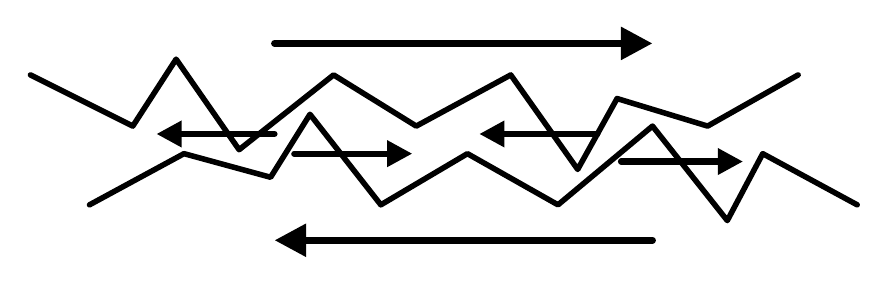
\begin{tikzpicture}[
    line cap=round,
    line join=round,
    >=Triangle
]

    % Top jagged surface profile
    \draw[line width=2pt] 
        (0.0, 2.2) -- 
        (1.3, 1.55) -- 
        (1.85, 2.4) -- 
        (2.65, 1.25) -- 
        (3.85, 2.2) -- 
        (4.9, 1.55) -- 
        (6.1, 2.2) -- 
        (6.95, 1.0) -- 
        (7.45, 1.9) -- 
        (8.6, 1.55) -- 
        (9.75, 2.2);

    % Bottom jagged surface profile
    \draw[line width=2pt] 
        (0.75, 0.55) -- 
        (1.95, 1.2) -- 
        (3.05, 0.9) -- 
        (3.55, 1.7) -- 
        (4.45, 0.55) -- 
        (5.55, 1.2) -- 
        (6.7, 0.55) -- 
        (7.9, 1.55) -- 
        (8.85, 0.35) -- 
        (9.3, 1.2) -- 
        (10.5, 0.55);

    % Macroscopic motion arrows (top and bottom)
    \draw[->, line width=2.5pt, arrows={-Triangle[length=4mm, width=4mm]}] 
        (3.1, 2.6) -- (7.9, 2.6);
    \draw[->, line width=2.5pt, arrows={-Triangle[length=4mm, width=4mm]}] 
        (7.9, 0.1) -- (3.1, 0.1);

    % Local resistance / force arrows between asperities
    % 1. Left-pointing arrow (upper left)
    \draw[->, line width=2.2pt, arrows={-Triangle[length=3.2mm, width=3.2mm]}] 
        (3.1, 1.45) -- (1.6, 1.45);
        
    % 2. Right-pointing arrow (lower left-center)
    \draw[->, line width=2.2pt, arrows={-Triangle[length=3.2mm, width=3.2mm]}] 
        (3.35, 1.2) -- (4.85, 1.2);
        
    % 3. Left-pointing arrow (upper right-center)
    \draw[->, line width=2.2pt, arrows={-Triangle[length=3.2mm, width=3.2mm]}] 
        (7.2, 1.45) -- (5.7, 1.45);
        
    % 4. Right-pointing arrow (lower right)
    \draw[->, line width=2.2pt, arrows={-Triangle[length=3.2mm, width=3.2mm]}] 
        (7.5, 1.1) -- (9.05, 1.1);

\end{tikzpicture}
                }
                
                \vspace{0.5em}
                {\tiny \textbf{Adapted from:} \href{https://commons.wikimedia.org/wiki/File:Friction_surface_microstructure.png}{CaoHao}, \href{http://creativecommons.org/licenses/by-sa/3.0/}{CC BY-SA 3.0}, via Wikimedia Commons, converted to TikZ format\par}
            \end{figure}
        \end{column}
    \end{columns}
\end{frame}

\begin{frame}
	\frametitle{Mechanical Motion}

    \begin{columns}
        \begin{column}{0.48\linewidth}
            \begin{itemize}[<+- | alert@+>]
                \item Movement = friction
                \item Friction = wear + heat
            \end{itemize}
        \end{column}
        \begin{column}{0.48\linewidth}
            \shadowpic[]{\linewidth}{A three-dimensional illustration showing two rectangular blocks in contact along jagged, microscopically rough surfaces against a white background, with a translucent blue-gray upper block resting atop a translucent orange-brown lower block so their irregular peaks and valleys interlock.}{\textbf{Attribution:} \href{https://commons.wikimedia.org/wiki/File:Friction_between_surfaces.jpg}{CaoHao}, \href{http://creativecommons.org/licenses/by-sa/4.0/}{CC BY-SA 4.0}, via Wikimedia Commons}{Friction_between_surfaces}
        \end{column}
    \end{columns}
\end{frame}

\begin{frame}
	\frametitle{Surface Friction}

    \begin{columns}
        \begin{column}{0.48\linewidth}
            \begin{itemize}[<+- | alert@+>]
                \item Smoother surface = less friction = higher speed/load
            \end{itemize}
        \end{column}
        \begin{column}{0.48\linewidth}
            \hexpic[]{0.75\linewidth}{A close-up photograph of a steel ball bearing resting on a light gray surface, showing its polished inner and outer rings with a ring of spherical steel balls held evenly spaced inside a riveted metal cage.}{\textbf{Attribution:} \href{https://commons.wikimedia.org/wiki/File:Ball_bearing.jpg}{Solaris2006}, \href{http://creativecommons.org/licenses/by-sa/3.0/}{CC BY-SA 3.0}, via Wikimedia Commons}{Ball_bearing}
        \end{column}
    \end{columns}
\end{frame}

\begin{frame}
	\frametitle{Lubrication}

    \shadowpic[]{\linewidth}{A diagram of laminar shear flow between two horizontal gray plates separated by a vertical gap height h, showing a bottom stationary plate and a top moving plate of length or area A pulled to the right by a blue force arrow labeled F, with a blue triangular linear velocity profile labeled Vx increasing from zero at the bottom to maximum at the top, a red vertical segmented column representing shear stress labeled tau xy, and a three-dimensional xyz coordinate axes legend at the bottom left.}{\textbf{Attribution:} \href{https://commons.wikimedia.org/wiki/File:Pressure_driven_laminar_flow_between_on_fixed_plate_and_top_moving_plate_with_shear_stress.png}{MiltonOrlandoUSF}, \href{http://creativecommons.org/licenses/by-sa/4.0/}{CC BY-SA 4.0}, via Wikimedia Commons}{Pressure_driven_laminar_flow}

    \vspace{0.5em}
    {\footnotesize Lubrication helps, but surface finish \emph{still} limits speeds/loads. There are shear forces and friction within the fluid itself, both of which create heat.\par}
\end{frame}

\begin{frame}
	\frametitle{Friction May Not Be a Bad Thing}

    \begin{columns}
        \begin{column}{0.48\linewidth}
            \begin{itemize}[<+- | alert@+>]
                \item Friction is why a small boat can pull a massive container ship
                \item Imagine pulling the same ship on land\dots
            \end{itemize}
        \end{column}
        \begin{column}{0.48\linewidth}
            \shadowpic[]{\linewidth}{A red-hulled cargo ship with three white deck cranes and a white rear superstructure sits in calm gray harbor water under an overcast sky, assisted by two tugboats at its bow and stern in front of low port buildings and a tall red-and-white lattice tower.}{\textbf{Attribution:} \href{https://commons.wikimedia.org/wiki/File:Ship_Pietersgracht_with_tugboats_in_Saint_Nazaire_harbour_02.jpg}{Hellotheworld}, \href{http://creativecommons.org/licenses/by-sa/4.0/}{CC BY-SA 4.0}, via Wikimedia Commons}{Ship_Pietersgracht_with_tugboats_in_Saint_Nazaire_harbour_02}
        \end{column}
    \end{columns}
\end{frame}

\subsection{Surface Finish as a Condition}

\begin{frame}
	\frametitle{Condition}

    \begin{columns}
        \begin{column}{0.48\linewidth}
            \begin{itemize}[<+- | alert@+>]
                \item Surface finish is a \emph{condition}
                \item Cannot be specified as a linear dimension
                \item Special instruments/units of measure defined to be able to specify/measure
            \end{itemize}
        \end{column}
        \begin{column}{0.48\linewidth}
            \shadowpic[]{\linewidth}{A close-up laser profilometry scan showing red vertical interference fringes across a metal surface, with a white horizontal arrow pointing from the left to a small dark circular corrosion pit near the center where the parallel lines curve and distort around the depression.}{\textbf{Attribution:} \href{https://commons.wikimedia.org/wiki/File:Laser_profilometry_-_pitting_corrosion.png}{Koz5000}, \href{http://creativecommons.org/licenses/by-sa/4.0/}{CC BY-SA 4.0}, via Wikimedia Commons}{Laser_profilometry_-_pitting_corrosion}
        \end{column}
    \end{columns}
\end{frame}

\begin{frame}
	\frametitle{Nominal Surface}

    \begin{columns}
        \begin{column}{0.48\linewidth}
            \begin{itemize}[<+- | alert@+>]
                \item Reference plane from which surface measurements will be taken
                \item Theoretically perfect surface (solid model, drawing, etc.)
            \end{itemize}
        \end{column}
        \begin{column}{0.48\linewidth}
            \shadowpic[]{\linewidth}{A three-dimensional CAD rendering of two aligned gray keyed shafts separated by a small gap, each fitted with a cylindrical hub and toothed sprocket facing each other and secured by a set screw against a light gray background.}{}{ChainCoupling}
        \end{column}
    \end{columns}
\end{frame}

\begin{frame}
	\frametitle{Surface Deviations}

    \begin{columns}
        \begin{column}{0.48\linewidth}
            \begin{itemize}[<+- | alert@+>]
                \item{Departures from the nominal (theoretically perfect) surface}
                    \begin{itemize}
                        \item{Flaws}
                        \item{Waviness}
                        \item{Roughness}
                        \item{Lay}
                        \item{Profile}
                    \end{itemize}
            \end{itemize}
        \end{column}
        \begin{column}{0.48\linewidth}
            \begin{figure}
                \centering
                \resizebox{\linewidth}{!}{
                    \begin{tikzpicture}[
    american, 
    >={Latex[length=5mm, width=2mm]},
    alt={A horizontal diagram comparing an actual rough surface profile to its ideal nominal profile. A jagged blue line runs horizontally across the center, oscillating slightly above and below a straight horizontal dashed red line. A thin red curved arrow points from the middle of the dashed red line upward and to the right to the text label Nominal Surface.}
    ]

    \draw[
        LakeBlue,
        ultra thick,
        decorate, 
        decoration={
            random steps,
            segment length=3pt,
            amplitude=2pt
        }
    ]
    (0,0)
    -- (5,0);

    \draw[
        BakerADARed,
        dashed
    ]
    (0,0)
    -- (5,0)
    coordinate[midway](label);

    \draw[
        BakerADARed,
        thin,
        <-
    ]
    (label)
    to[out=45, in=180]
    ++(2,1)
    node[
        text=BakerBlack,
        anchor=west,
        align=left
    ]
    {Nominal\\Surface};

\end{tikzpicture}
                }
            \end{figure}
        \end{column}
    \end{columns}
\end{frame}

\begin{frame}
	\frametitle{Surface Flaws}
    
    \begin{columns}
        \begin{column}{0.48\linewidth}
            \begin{itemize}[<+- | alert@+>]
                \item Irregularities that occur at one place or at relatively infrequent intervals
                    \begin{itemize}
                        \item Scratches
                        \item Ridges
                        \item Hollows
                        \item Cracks 
                    \end{itemize}
            \end{itemize}
        \end{column}
        \begin{column}{0.48\linewidth}
            \shadowpic[]{\linewidth}{A three-dimensional surface topography map of a deep scratch across a flat glass surface, spanning 600 micrometers on both horizontal axes and up to 9.41 micrometers on the vertical axis, with the surrounding smooth surface colored pale pink and the deep groove shaded in a rainbow gradient from red and yellow down to dark blue at its deepest trough, crossed by a black and blue profile measurement line and accompanied by a vertical height color scale on the right.}{\textbf{Attribution:} \href{https://commons.wikimedia.org/wiki/File:Scratch_on_glass_surface,_3D_topography_(26711616455).jpg}{ZEISS Microscopy from Germany}, \href{http://creativecommons.org/licenses/by-sa/2.0/}{CC BY-SA 2.0}, via Wikimedia Commons}{Scratch_on_glass_surface,_3D_topography_(26711616455)}
        \end{column}
    \end{columns}
\end{frame}

\begin{frame}
	\frametitle{Waves}

    \begin{columns}
        \begin{column}{0.48\linewidth}
            \begin{itemize}[<+- | alert@+>]
                \item Recurrent or random irregularities on a surface in the form of waves
                \item Peak-to-peak 0.030" to several inches
            \end{itemize}
        \end{column}
        \begin{column}{0.48\linewidth}
            \begin{figure}
                \centering
                \resizebox{\linewidth}{!}{
                    \begin{tikzpicture}[
    american, 
    >={Latex[length=5mm, width=2mm]},
    alt={}
    ]

    \draw[
        LakeBlue,
        ultra thick,
        decorate, 
        decoration={
            coil,
            aspect=0,
            amplitude=3pt
        }
    ]
    (0,0)
    -- (5,0);

    \draw[
        BakerADARed,
        dashed
    ]
    (0,0)
    -- (5,0)
    coordinate[midway](label);

\end{tikzpicture}
                }
            \end{figure}
        \end{column}
    \end{columns}
\end{frame}

\begin{frame}
	\frametitle{Roughness (1 of 2)}

    \begin{columns}
        \begin{column}{0.48\linewidth}
            \begin{itemize}[<+- | alert@+>]
                \item Relatively finely spaced irregularities superimposed on a flat or wavy surface             
                \item Roughness measurement deals with these irregularities
            \end{itemize}
        \end{column}
        \begin{column}{0.48\linewidth}
            \shadowpic[]{\linewidth}{A black-and-white technical cross-section diagram showing how stylus tip radius affects surface roughness measurement, with a jagged solid line and diagonal hatching representing the actual rough surface profile overlaid by two traced paths, a dashed line closely following the valleys for a 2.5 micrometer radius stylus and a dotted line bridging across the peaks for a 12.5 micrometer radius stylus, accompanied by an Italian legend at the bottom translating to path followed by a stylus with radius 2.5 micrometers and path followed by a stylus with radius 12.5 micrometers.}{\textbf{Attribution:} \href{https://commons.wikimedia.org/wiki/File:STILO3.jpg}{Lucabu images}, CC0, via Wikimedia Commons}{STILO3}
        \end{column}
    \end{columns}
\end{frame}

\begin{frame}
	\frametitle{Roughness (2 of 2)}

    \begin{columns}
        \begin{column}{0.48\linewidth}
            \begin{itemize}[<+- | alert@+>]
                \item Machining--produced by cutting action of the tool
                \item Abrasive operations--cutting action of the grains
            \end{itemize}
        \end{column}
        \begin{column}{0.48\linewidth}
            \shadowpic[]{\linewidth}{A black-and-white technical cross-section diagram showing how stylus tip radius affects surface roughness measurement, with a jagged solid line and diagonal hatching representing the actual rough surface profile overlaid by two traced paths, a dashed line closely following the valleys for a 2.5 micrometer radius stylus and a dotted line bridging across the peaks for a 12.5 micrometer radius stylus, accompanied by an Italian legend at the bottom translating to path followed by a stylus with radius 2.5 micrometers and path followed by a stylus with radius 12.5 micrometers.}{\textbf{Attribution:} \href{https://commons.wikimedia.org/wiki/File:STILO3.jpg}{Lucabu images}, CC0, via Wikimedia Commons}{STILO3}
        \end{column}
    \end{columns}
\end{frame}

\begin{frame}
	\frametitle{Profile}

    \begin{columns}
        \begin{column}{0.48\linewidth}
            \begin{itemize}[<+- | alert@+>]
                \item A contour of the roughness and waviness of the surface
            \end{itemize}
        \end{column}
        \begin{column}{0.48\linewidth}
            \shadowpic[]{\linewidth}{A black-and-white technical cross-section diagram showing how stylus tip radius affects surface roughness measurement, with a jagged solid line and diagonal hatching representing the actual rough surface profile overlaid by two traced paths, a dashed line closely following the valleys for a 2.5 micrometer radius stylus and a dotted line bridging across the peaks for a 12.5 micrometer radius stylus, accompanied by an Italian legend at the bottom translating to path followed by a stylus with radius 2.5 micrometers and path followed by a stylus with radius 12.5 micrometers.}{\textbf{Attribution:} \href{https://commons.wikimedia.org/wiki/File:STILO3.jpg}{Lucabu images}, CC0, via Wikimedia Commons}{STILO3}
        \end{column}
    \end{columns}
\end{frame}

\begin{frame}
	\frametitle{Surface Lay (1 of 2)}

    \begin{columns}
        \begin{column}{0.48\linewidth}
            \begin{itemize}[<+- | alert@+>]
                \item Direction of the predominant surface pattern
            \end{itemize}
        \end{column}
        \begin{column}{0.48\linewidth}
            \shadowpic[]{\linewidth}{A technician wearing a dark flat cap, safety glasses, earplugs, a tan work shirt, and a black apron stands at a workshop bench holding a small round metal specimen on a light blue lapping surface next to a gray metal fixture block and assorted shop bottles and tools.}{\textbf{Attribution:} Dori Whipple, Public domain, via \href{https://www.dvidshub.net/image/3659435/machinists-create-scratch-production-plant-barstow}{U.S. Department of War Digital Visual Information Distribution System}}{3659435}
        \end{column}
    \end{columns}
\end{frame}

\begin{frame}
	\frametitle{Surface Lay (2 of 2)}

    \begin{columns}
        \begin{column}{0.48\linewidth}
            \begin{itemize}[<+- | alert@+>]
                \item Milling, turning, grinding -- definite direction of lay
                \item Lapping -- random pattern (multi-directional)
            \end{itemize}
        \end{column}
        \begin{column}{0.48\linewidth}
            \shadowpic[]{\linewidth}{A technician wearing a dark flat cap, safety glasses, earplugs, a tan work shirt, and a black apron stands at a workshop bench holding a small round metal specimen on a light blue lapping surface next to a gray metal fixture block and assorted shop bottles and tools.}{\textbf{Attribution:} Dori Whipple, Public domain, via \href{https://www.dvidshub.net/image/3659435/machinists-create-scratch-production-plant-barstow}{U.S. Department of War Digital Visual Information Distribution System}}{3659435}
        \end{column}
    \end{columns}
\end{frame}

\begin{frame}
	\frametitle{Surface Finish Video}

    \centering
    {\large \href{https://www.youtube.com/watch?v=6ZFT4nBEEFY}{Machined Surface Finishes (Metal Machining Video 6)}\par}

    \vspace{0.5em}
    {\footnotesize \href{https://www.youtube.com/watch?v=6ZFT4nBEEFY}{https://www.youtube.com/watch?v=6ZFT4nBEEFY}\par}

    \vspace{0.5em}
    {\tiny Video \textcopyright{} Sofeast via YouTube.com\par}
\end{frame}

\section{Surface Finish Specification}

\begin{frame}
	\frametitle{Surface Finish}

    \begin{figure}
        \centering
        \resizebox{\linewidth}{!}{
            \begin{tikzpicture}[
    american, 
    >={Latex[length=5mm, width=2mm]},
    alt={An engineering drawing showing a stepped cylindrical shaft in side view on the left and end view on the right, crossed by a horizontal dashed red centerline extending through both views and a vertical dashed red centerline bisecting the end view. In the side view, a large black rectangle connects on the right to a smaller black rectangle, with a surface finish symbol resting on top of the smaller step displaying a roughness value of 16 on the left, a waviness height of 0.005 above the horizontal bar, and a perpendicular lay symbol followed by a sampling length of 0.030 on the right. To the right of the side view, the end view consists of two concentric black circles corresponding to the diameters of the two stepped sections.}
    ]

    \node[
        draw=BakerBlack,
        ultra thick,
        minimum height=3.5cm,
        minimum width=8cm
    ](bigD)
    at (0,0)
    {};

    \node[
        draw=BakerBlack,
        ultra thick,
        anchor=west,
        minimum height=2cm,
        minimum width=4cm
    ](smallD)
    at (bigD.east)
    {};

    \pic at (smallD.north) {roughness={16}{0.005}{$\perp$0.030}};

    \node[
        draw=BakerBlack,
        anchor=west,
        circle,
        minimum size=3.5cm
    ](lView)
    at ($(smallD.east)+(2cm,0)$)
    {};

    \node[
        draw=BakerBlack,
        circle,
        minimum size=2cm
    ](lViewS)
    at (lView.center)
    {};

    \draw[
        BakerADARed,
        dashed,
        shorten <=-1cm,
        shorten >=-1cm
    ]
    (bigD.west)
    -- (lView.east);

    \draw[
        BakerADARed,
        dashed,
        shorten <=-1cm,
        shorten >=-1cm
    ]
    (lView.north)
    -- (lView.south);

\end{tikzpicture}
        }

        \vspace{0.5em}
        {\footnotesize Surface finish has a specific set of symbols on engineering drawings.\par}
    \end{figure}
\end{frame}

\begin{frame}
	\frametitle{Surface Finish Symbol}

    \begin{figure}
        \centering
        \resizebox{\linewidth}{!}{
            \begin{tikzpicture}[
    american, 
    >={Latex[length=5mm, width=2mm]},
    alt={An engineering drawing showing a stepped cylindrical shaft in side view on the left and end view on the right, crossed by a horizontal dashed red centerline extending through both views and a vertical dashed red centerline bisecting the end view. In the side view, a large black rectangle connects on the right to a smaller black rectangle, with a surface finish symbol resting on top of the smaller step displaying a roughness value of 16 on the left, a waviness height of 0.005 above the horizontal bar, and a perpendicular lay symbol followed by a sampling length of 0.030 on the right. To the right of the side view, the end view consists of two concentric black circles corresponding to the diameters of the two stepped sections.}
    ]

    \pic (symb) at (smallD.north) {roughness={16}{0.005}{$\perp$0.030}};

    \draw[
        UpNorthGreen,
        <-
    ]
    (symb-topValue.north east)
    to[out=45, in=180]
    ++(1,1)
    node[
        text=BakerBlack,
        align=left,
        anchor=west
    ]{Waviness\\height};

    \draw[
        UpNorthGreen,
        <-
    ]
    (symb-leftValue.north west)
    to[out=135, in=0]
    ++(-1,1)
    node[
        text=BakerBlack,
        anchor=east,
        align=right
    ]{Roughness\\height (\SI{}{\micro in})};

    \draw[
        UpNorthGreen,
        <-
    ]
    (symb-rightValue.south east)
    to[out=330, in=180]
    ++(2,-0.5)
    node[
        text=BakerBlack,
        anchor=west,
        align=left
    ]{Roughness\\width};

    \draw[
        UpNorthGreen,
        <-
    ]
    ($(symb-rightValue.south west)+(0.25cm,0)$)
    to[out=270, in=180]
    ++(1,-1)
    node[
        text=BakerBlack,
        anchor=west,
        align=left
    ]{Direction\\of lay};
\end{tikzpicture}
        }
    \end{figure}
\end{frame}

\begin{frame}
	\frametitle{Surface Finish Specification}

    \begin{figure}
        \centering
        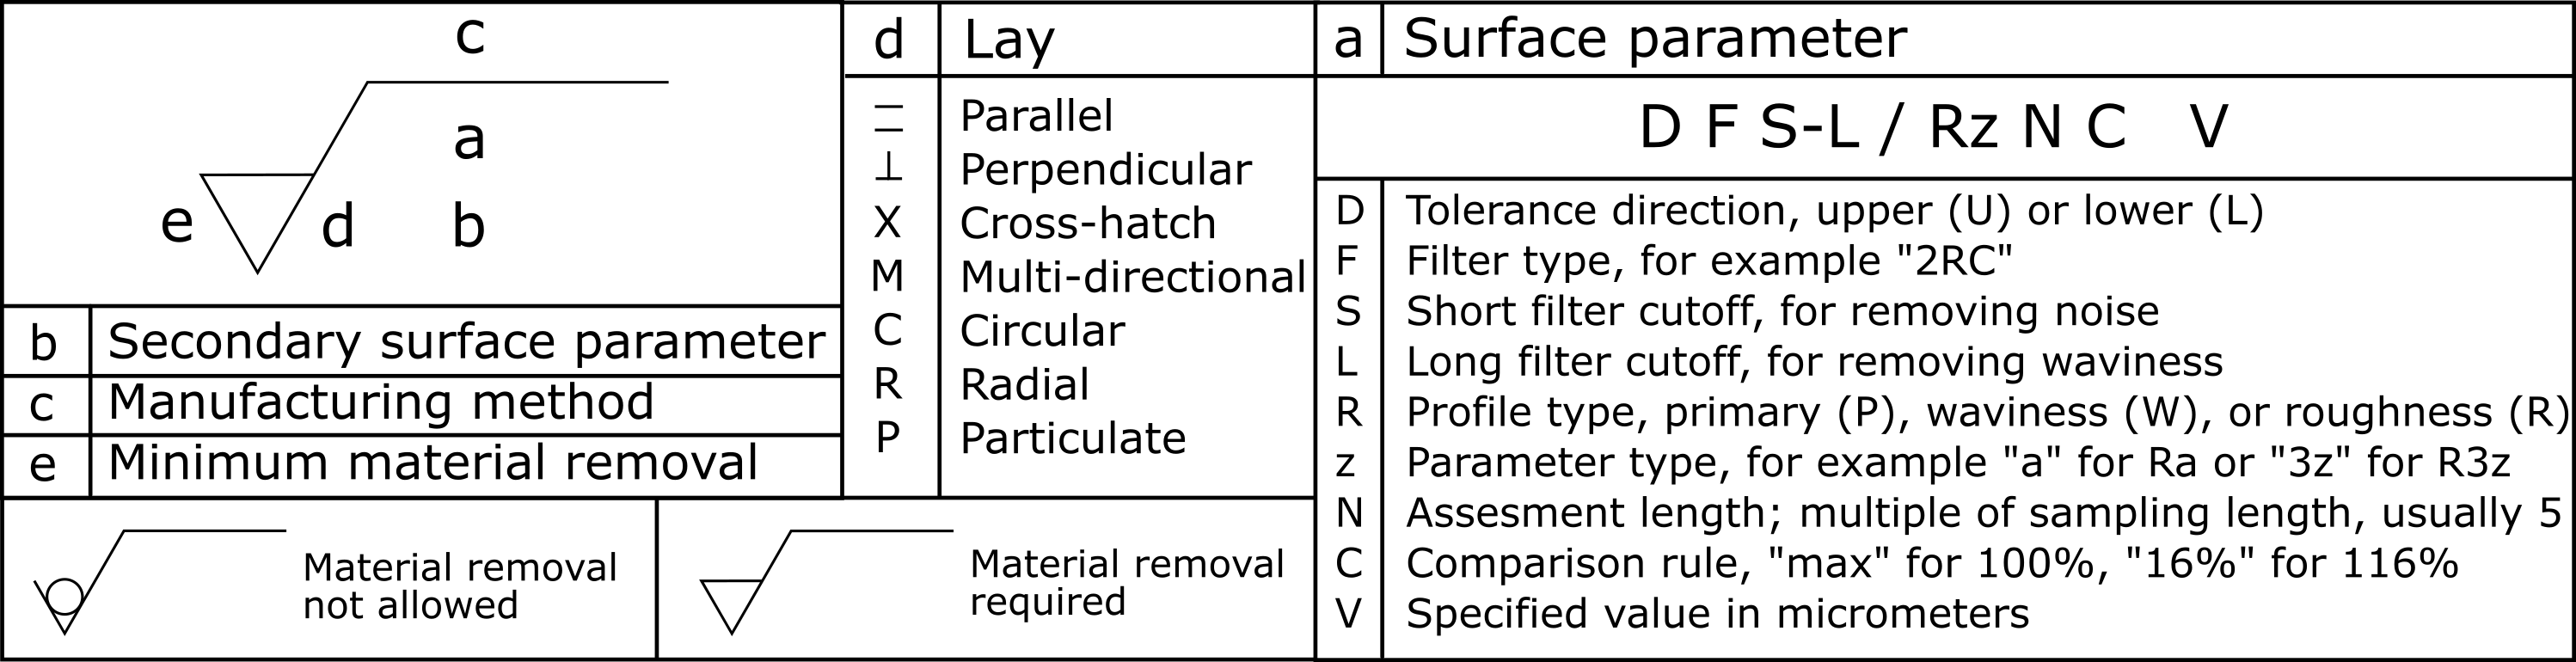
\includegraphics[width=\linewidth, alt={A black-and-white technical schematic grid illustrating standard engineering surface finish symbols and layout boxes against a white background, featuring a closed-triangle material-removal-required symbol with a horizontal extension bar in the upper left cell, parallel and perpendicular lay direction symbols in a narrow vertical column near the center, and two smaller surface texture symbols at the bottom left showing a circle inside a V-shape for material removal prohibited and a closed triangle for material removal required, alongside blank rectangular table cells on the right.}]{Surface_finish_specification2}

        \vspace{0.5em}
        {\tiny \textbf{Attribution:} \href{https://commons.wikimedia.org/wiki/File:Surface_finish_specification2.svg}{Surface\_finish\_specification.svg: Emok derivative work: Wizard191}, \href{http://creativecommons.org/licenses/by-sa/3.0/}{CC BY-SA 3.0}, via Wikimedia Commons\par}
    \end{figure}
\end{frame}

\begin{frame}
	\frametitle{Lay Direction Example}

    \begin{columns}
        \begin{column}{0.48\linewidth}
            \begin{figure}
                \centering
                \resizebox{\linewidth}{!}{
                    \begin{tikzpicture}[
    american, 
    >={Latex[length=5mm, width=2mm]},
    alt={An engineering diagram showing a rectangular prism in isometric perspective at the top, with its top surface covered in closely spaced thin red parallel lines running front-to-back along its length to indicate surface lay direction. Below the isometric block are two two-dimensional orthographic views side by side: a shorter black rectangle labeled Front on the left, and a wider black rectangle labeled Side on the right. Resting on the top edge of the Side view is a black surface finish symbol displaying a parallel lay symbol to the right of its bar, indicating that the surface texture runs parallel to the plane of the side view.}
    ]

    \def\width{4}
    \def\height{1}
    \def\depth{5}

    \def\step{0.25}
    \pgfmathsetmacro{\second}{2 * \step}
    \pgfmathsetmacro{\xmax}{\width - \step}

    \node[
        draw=BakerBlack,
        ultra thick,
        anchor=north west,
        minimum height=\height cm,
        minimum width=\width cm
    ](front)
    at (0,0)
    {};

    \draw[
        BakerBlack,
        ultra thick
    ]
    (0,0)
    -- (30:\depth)
    -- ++(\width cm,0)
    -- (front.north east);

    \draw[
        BakerBlack,
        ultra thick
    ]
    (front.south east)
    -- ++(30:\depth)
    -- ++(0,\height);

    \foreach \x in {\step,\second,...,\xmax}
    {
        \draw[
            BakerADARed,
            ultra thin
        ]
        (\x,0)
        -- ++(30:\depth);
    }

    \begin{scope}[xshift=-1cm, yshift=-2cm]

        \node[
            draw=BakerBlack,
            text=BakerBlack,
            ultra thick,
            anchor=north west,
            minimum height=\height cm,
            minimum width=\width cm
        ](frontV)
        at (0,0)
        {Front};

        \node[
            draw=BakerBlack,
            text=BakerBlack,
            ultra thick,
            anchor=north west,
            minimum height=\height cm,
            minimum width=\depth cm
        ](sideV)
        at ($(frontV.north east)+(1cm,0)$)
        {Side};

        \pic at (sideV.north) {roughness={}{}{$\parallel$}};

    \end{scope}


\end{tikzpicture}
                }

                \vspace{0.5em}
                {\footnotesize Parallel to edge indicated\par}
            \end{figure}
        \end{column}
        \begin{column}{0.48\linewidth}
            \begin{figure}
                \centering
                \resizebox{\linewidth}{!}{
                    \begin{tikzpicture}[
    american, 
    >={Latex[length=5mm, width=2mm]},
    alt={An engineering diagram showing a rectangular prism in isometric perspective at the top, with its top surface covered in closely spaced thin red parallel lines running left-to-right across its width to indicate surface lay direction. Below the isometric block are two two-dimensional orthographic views side by side: a shorter black rectangle labeled Front on the left, and a wider black rectangle labeled Side on the right. Resting on the top edge of the Side view is a black surface finish symbol displaying a perpendicular lay symbol to the right of its bar, indicating that the surface texture runs perpendicular to the plane of the side view.}
    ]

    \def\width{4}
    \def\height{1}
    \def\depth{5}

    \def\step{0.25}
    \pgfmathsetmacro{\second}{2 * \step}
    \pgfmathsetmacro{\dmax}{\depth - \step}

    \node[
        draw=BakerBlack,
        ultra thick,
        anchor=north west,
        minimum height=\height cm,
        minimum width=\width cm
    ](front)
    at (0,0)
    {};

    \draw[
        BakerBlack,
        ultra thick
    ]
    (0,0)
    -- (30:\depth)
    -- ++(\width cm,0)
    -- (front.north east);

    \draw[
        BakerBlack,
        ultra thick
    ]
    (front.south east)
    -- ++(30:\depth)
    -- ++(0,\height);

    \foreach \d in {\step,\second,...,\dmax}
    {
        \draw[
            BakerADARed,
            ultra thin
        ]
        (30:\d)
        -- ++(\width,0);
    }

    \begin{scope}[xshift=-1cm, yshift=-2cm]

        \node[
            draw=BakerBlack,
            text=BakerBlack,
            ultra thick,
            anchor=north west,
            minimum height=\height cm,
            minimum width=\width cm
        ](frontV)
        at (0,0)
        {Front};

        \node[
            draw=BakerBlack,
            text=BakerBlack,
            ultra thick,
            anchor=north west,
            minimum height=\height cm,
            minimum width=\depth cm
        ](sideV)
        at ($(frontV.north east)+(1cm,0)$)
        {Side};

        \pic at (sideV.north) {roughness={}{}{$\perp$}};

    \end{scope}

\end{tikzpicture}
                }

                \vspace{0.5em}
                {\footnotesize Perpendicular to edge indicated\par}
            \end{figure}
        \end{column}
    \end{columns}
\end{frame}

\section{Profilometers}

\begin{frame}
	\frametitle{Profilometer}

    \begin{columns}
        \begin{column}{0.48\linewidth}
            \begin{itemize}[<+- | alert@+>]
                \item Mechanical-electronic instrument for measuring surface roughness in microinch (\SI{}{\micro in}, 0.000001") 
            \end{itemize}
        \end{column}
        \begin{column}{0.48\linewidth}
            \shadowpic[]{0.75\linewidth}{A vintage Talysurf Model 2 surface roughness measuring instrument on display in a museum, featuring a heavy dark metal base with a vertical column and horizontal stylus arm, a wooden chart recorder box on the right, and electronic control units stored on the lower shelves of a wheeled wooden-topped cart in front of a wood-paneled partition.}{\textbf{Attribution:} \href{https://commons.wikimedia.org/wiki/File:Talysurf,_Snibston.jpg}{Andy Dingley}, \href{http://creativecommons.org/licenses/by-sa/3.0/}{CC BY-SA 3.0}, via Wikimedia Commons}{Talysurf,_Snibston}
        \end{column}
    \end{columns}
\end{frame}

\begin{frame}
	\frametitle{Profilometer Setup}

    \begin{columns}
        \begin{column}{0.48\linewidth}
            \begin{itemize}[<+- | alert@+>]
                \item{Part placed under measurement head}
                    \begin{itemize}
                        \item{Some heads are motorized}
                        \item{Some are moved by hand over part}
                    \end{itemize}
                \item{Skid or stud rides on part}
                    \begin{itemize}
                        \item{Skid/stud sets the reference surface}
                    \end{itemize}
            \end{itemize}
        \end{column}
        \begin{column}{0.48\linewidth}
            \shadowpic[]{0.875\linewidth}{A close-up photograph of a Taylor-Hobson Surtronic 3P portable surface roughness profilometer resting on a patterned metal surface plate, featuring a rectangular light gray display and control unit on the upper right with rotary dials and a small screen, connected to a vertical black adjustment column and a silver cylindrical stylus arm extending forward to rest its tip on a small metal cylinder seated atop a grooved dark V-block on the lower left.}{\textbf{Attribution:} \href{https://commons.wikimedia.org/wiki/File:Profilometr_Surtronic_3P.jpg}{Rrudzik}, CC0, via Wikimedia Commons}{Profilometr_Surtronic_3P}
        \end{column}
    \end{columns}
\end{frame}

\begin{frame}
	\frametitle{Profilometer Measurement}

    \shadowpic[]{0.5\linewidth}{A black-and-white technical schematic illustrating a skidded stylus profilometer traversing a rough surface from left to right as indicated by a horizontal arrow. In the upper section, a rounded mechanical skid slides over the peaks of a jagged cross-hatched profile labeled SUPERFICIE, while an adjacent pointed black stylus tip probes into the surface valleys to measure height variations. In the lower section, a wavy continuous line labeled GRAFICO displays the resulting recorded roughness profile below the physical surface.}{\textbf{Attribution:} \href{https://commons.wikimedia.org/wiki/File:PATTINO3.jpg}{Lucabu}, CC0, via Wikimedia Commons}{PATTINO3}

    \centering
    \vspace{0.5em}
    {\footnotesize A skid or stud rides on the surface, setting the reference surface. The stylus then rides on the surface--deviations in the stylus height are the recorded measurement.\par}
\end{frame}

\begin{frame}
	\frametitle{Profilometer Limits}

    \shadowpic[]{0.75\linewidth}{A black-and-white technical cross-section diagram showing how stylus tip radius affects surface roughness measurement, with a jagged solid line and diagonal hatching representing the actual rough surface profile overlaid by two traced paths, a dashed line closely following the valleys for a 2.5 micrometer radius stylus and a dotted line bridging across the peaks for a 12.5 micrometer radius stylus, accompanied by an Italian legend at the bottom translating to path followed by a stylus with radius 2.5 micrometers and path followed by a stylus with radius 12.5 micrometers.}{\textbf{Attribution:} \href{https://commons.wikimedia.org/wiki/File:STILO3.jpg}{Lucabu images}, CC0, via Wikimedia Commons}{STILO3}

    \centering
    \vspace{0.5em}
    {\footnotesize The stylus size limits the how accurate the profilometer can be--it's simply too big to fit in \emph{all} of the valleys.\par}
\end{frame}

\begin{frame}
    \frametitle{Profilometer Videos}

    \centering
    {\large \href{https://www.youtube.com/watch?v=mQg7TPmhqfk}{Introduction to stylus profilometers}\par}

    \vspace{0.5em}
    {\footnotesize \href{https://www.youtube.com/watch?v=mQg7TPmhqfk}{https://www.youtube.com/watch?v=mQg7TPmhqfk}\par}

    \vspace{0.5em}
    {\tiny Video \textcopyright{} Surface Metrology Guide via YouTube.com\par}

    \vspace{0.5in}

    {\large \href{https://www.youtube.com/watch?v=MaQyQUxxWKo}{Profilometer}\par}

    \vspace{0.5em}
    {\footnotesize \href{https://www.youtube.com/watch?v=MaQyQUxxWKo}{https://www.youtube.com/watch?v=MaQyQUxxWKo}\par}

    \vspace{0.5em}
    {\tiny Video \textcopyright{} machinist. todd via YouTube.com\par}
\end{frame}

\begin{frame}
	\frametitle{Profilometer Drawbacks}

    \begin{itemize}[<+- | alert@+>]
        \item We're dragging a metal stylus across the part
        \item If the stylus is soft (it isn't) it'll wear down and not be able to ride in the surface imperfections
        \item If the stylus is hard (it is) we're dragging a \emph{hard} metal sylus across the part
        \item The potential to add surface imperfections while taking the measurement
    \end{itemize}
\end{frame}

\section{Optical Profilometers}

\begin{frame}
	\frametitle{Optical Profilometer (1 of 2)}

    \begin{columns}
        \begin{column}{0.48\linewidth}
            \begin{itemize}[<+- | alert@+>]
                \item New technology allows non-contact profilometers
                    \begin{itemize}
                        \item Laser scanning
                        \item Simpler light sources
                    \end{itemize}
            \end{itemize}
        \end{column}
        \begin{column}{0.48\linewidth}
            \shadowpic[]{0.75\linewidth}{A close-up photograph of a Nanovea PS50 non-contact optical profilometer against a light gray background, featuring a vertical cylindrical black optical sensor pen held in a blue anodized clamp on a black gantry frame with a braided silver fiber optic cable extending from the top, positioned directly above a small machined metal test sample resting on a square black stage framed in blue.}{\textbf{Attribution:} \href{https://commons.wikimedia.org/wiki/File:NANOVEA_PS50_Non-Contact_Optical_Profilometer.jpg}{Materials Science 1}, \href{https://creativecommons.org/licenses/by-sa/4.0}{CC BY-SA 4.0}, via Wikimedia Commons}{NANOVEA_PS50_Non-Contact_Optical_Profilometer}
        \end{column}
    \end{columns}
\end{frame}

\begin{frame}
	\frametitle{Optical Profilometer (1 of 2)}

    \begin{columns}
        \begin{column}{0.48\linewidth}
            \begin{itemize}[<+- | alert@+>]
                \item Light = no contact = no damage to part
                \item Capable of producing a full 3D image of the surface instead of just profile
            \end{itemize}
        \end{column}
        \begin{column}{0.48\linewidth}
            \shadowpic[]{0.75\linewidth}{A close-up photograph of a Nanovea PS50 non-contact optical profilometer against a light gray background, featuring a vertical cylindrical black optical sensor pen held in a blue anodized clamp on a black gantry frame with a braided silver fiber optic cable extending from the top, positioned directly above a small machined metal test sample resting on a square black stage framed in blue.}{\textbf{Attribution:} \href{https://commons.wikimedia.org/wiki/File:NANOVEA_PS50_Non-Contact_Optical_Profilometer.jpg}{Materials Science 1}, \href{https://creativecommons.org/licenses/by-sa/4.0}{CC BY-SA 4.0}, via Wikimedia Commons}{NANOVEA_PS50_Non-Contact_Optical_Profilometer}
        \end{column}
    \end{columns}
\end{frame}

\begin{frame}
	\frametitle{NANOVEA Non-Contact Profilometer Video}

    \centering
    {\large \href{https://www.youtube.com/watch?v=hw2YNwdWeLo}{Profilometer | 3D Non Contact Profilometry}\par}

    \vspace{0.5em}
    {\footnotesize \href{https://www.youtube.com/watch?v=hw2YNwdWeLo}{https://www.youtube.com/watch?v=hw2YNwdWeLo}\par}

    \vspace{0.5em}
    {\tiny Video \textcopyright{} NANOVEA via YouTube.com\par}
\end{frame}

\begin{frame}
	\frametitle{Optical Profilometer Surface Image}
    
    \shadowpic[]{0.75\linewidth}{A two-panel three-dimensional surface topography scan of a titanium nitride coating rendered in a rainbow height color map ranging from blue valleys to yellow and red peaks. On the left, an oblique view shows a square scan area measuring 0.841 millimeters by 0.841 millimeters with a maximum height of 8.07 micrometers, featuring a red rectangular highlight box in the center. On the right, a magnified view of the highlighted area shows flat-topped yellow plateaus with steep green and blue vertical sidewalls rising from deep blue valleys.}{\textbf{Attribution:} \href{https://commons.wikimedia.org/wiki/File:TiN_coating.jpg}{Somnath Bharech}, \href{https://creativecommons.org/licenses/by/4.0}{CC BY 4.0}, via Wikimedia Commons}{TiN_coating}
\end{frame}

\begin{frame}
    \centering
    {\Huge \textbf{\textcolor{BakerADARed}{Questions?}}}
\end{frame}

\begin{frame}
    \frametitle{Copyright Notice}
    
    {\scriptsize
    \PresTitle \textcopyright 2026 by Brad Peirson is licensed under Creative Commons Attribution-NonCommercial-ShareAlike 4.0 International (CC BY-NC-SA 4.0). To view a copy of the official license, visit \href{https://creativecommons.org/licenses/by-nc-sa/4.0/}{https://creativecommons.org/licenses/by-nc-sa/4.0/}.

    \vspace{0.5em}

    \textbf{Exceptions and Exclusions}

    \begin{itemize}
        \item[Baker College Branding \& Trademarks:]All Baker College logos, trademarks, wordmarks, seals, slide design templates, and proprietary branding elements contained in these materials are \textbf{EXCLUDED} from the CC BY-NC-SA 4.0 license. All rights are reserved by Baker College. Express written permission from Baker College is required for any use, copying, or redistribution of these elements.
        \item[Third-Party Media \& Content:] Any third-party images, graphics, diagrams, or external media incorporated in these materials are included under their respective original licenses or permissions and are individually attributed at their point of use. 
        \item[Original Author Content:] All unattributed figures, diagrams, text, code snippets, and media are original works created by the author and are licensed under the CC BY-NC-SA 4.0 license.
    \end{itemize}

    The appearance of U.S. Department of War (DoW) visual information does not imply or constitute DoW endorsement.
    \par}
\end{frame}

\end{document}

% \begin{frame}
%     \frametitle{Test Todo}

%     % Usage: \tikztodo[width]{height}{description/notes}
%     \tikztodo[0.7\textwidth]{4cm}{Convert block diagram of feedback loop}
% \end{frame}